\begin{pa} \label{PA:1.3}
Suppose that $f$ is the function given by the graph below and that $a$ and $a+h$ are the input values as labeled on the $x$-axis.  Use the graph in Figure~\ref{F:1.3.PA1} to answer the following questions.

\begin{figure}[h]
\begin{center}
\includegraphics{figures/1_3_PA1.eps}
\caption{Plot of $y = f(x)$ for Preview Activity~\ref{PA:1.3}.} \label{F:1.3.PA1}
\end{center}
\end{figure}
\ba
	\item Locate and label the points $(a,f(a))$ and $(a+h, f(a+h))$ on the graph.
	\item Construct a right triangle whose hypotenuse is the line segment from $(a,f(a))$ to \\ $(a+h,f(a+h))$.  What are the lengths of the respective legs of this triangle?
	\item What is the slope of the line that connects the points $(a,f(a))$ and $(a+h, f(a+h))$?
	\item Write a meaningful sentence that explains how the average rate of change of the function on a given interval and the slope of a related line are connected.
\ea
\end{pa} \afterpa